\section{Evaluation}
\label{sec:experiments}
%\todo[author=DSN,inline]{Have you described the architecture and hardware of the lab-based cloud data centre elsewhere in the paper? What processors, memories, storage, networking, etc you have on the machines?}
%\noindent We performed a number of experiments in a lab-based cloud data centre in order to evaluate the performance of our approach and support the assumption that we discussed in Section~\ref{sec:approach}. In this section we present the results from these experiments and discuss them. Specifically, in this section we attempt to answer the research questions as listed in section~\ref{sec:research-questions}. In section~\ref{sec:experimental_setup} we explain the experimental set-up or testbed set-up that is used to perform the experiments. 
\noindent We performed a number of experiments to evaluate the performance of RADS. The experiments can be classified into: lab-based and real-world. The lab-based experiments were performed in an OpenStack\footnote{https://www.openstack.org} based Cloud data centre, which hosted two representative Cloud applications drawn from the CloudSuite\footnote{http://cloudsuite.ch} benchmark suite. The real-world experiments were carried out on the real-world workload traces~\cite{workloadCCGRID:2015} collected from a Cloud data centre named Bitbrains\footnote{https://www.solvinity.com}.
In this section we present the results from these experiments and discuss them. 
Specifically, we attempt to answer the following research questions: 
%Specifically, in this section we attempt to answer the research questions listed in section~\ref{sec:research-questions}. 
%In section~\ref{sec:experimental_setup} we explain the experimental set-up or testbed set-up that is used to perform the real-time experiments. 
%Section~\ref{sec:behavioural_analysis} presents the behavioural pattern analysis of various cloud applications under both normal and security attack conditions. Finally, we evaluate the effectiveness and efficiency of RAIDS in Section~\ref{sec:raids-performance} and section~\ref{sec:raids-efficiency} respectively. 
%\subsection{Research Questions}
%\label{sec:research-questions}
%\noindent The evaluation process aims to answer the following research questions:
\begin{enumerate}[{(1)}]
%\item Do the experimental results obtained from running various cloud applications verify the problems identified (in Section~\ref{sec:problem_definition}) in the existing statistical approaches used for IDSs. 
%\item Does the experimental evidence support our \textbf{assumption} that we made in Section~\ref{sec:approach}?
	%\todo[author=DSN,inline]{You need to restate this assumption here, the reader may not be able to remember everything!}
%\item Does using a combination of the average and the standard deviation of the raw data solves the problems identified in Section~\ref{sec:problem_definition}?
%Does using a combination of the average and the standard deviation of the raw data solves this problem?}
%\item Are there cases when the state-of-the-art average and entropy based techniques fail in successfully differentiating between cloud applications' normal behavioural pattern that may carry instantaneous spikes and anomalous behavioural pattern that arise due to the security attacks? Does using a combination of the average and the standard deviation of the raw data solves this problem?
%\item What is the accuracy of RAIDS while it uses a combination of average and standard deviation of the raw data as the data pre-processing approach? Does this accuracy outperform the accuracy that is achieved by using state-of-the art average and entropy based approaches?
%\item What is the performance of RAIDS in detecting Cloud intru- sions in real-time? Does RAIDS achieves better performance while using the proposed data pre-processing approach which is based on the average and the standard deviation than that achieved when using state-of-the-art data pre-processing approaches for Cloud IDSs which are based on either the average or the entropy?
\item Can RADS accurately detect Cloud anomalies occurring due to DDoS and cryptomining attacks in real-time? 
\item Can RADS window-based time series analysis outperform the state-of-the-art average and entropy based analyses in terms of accuracy and false positive rate? 
%\item Does the proposed data pre-processing approach which is based on the average and the standard deviation achieves better performance compared to the state-of-the-art data pre-processing approaches for Cloud IDSs which are based on either the average or the entropy? 
%\item While operating in real-time, how much overhead does RAIDS impose on the hosting node resources and how long does RAIDS take to complete the training and the intrusion detection process? 
\item Can RADS be used as a lightweight tool in terms of consuming minimal computing resources and processing time in a Cloud data centre? %used as a lightweight tool for detecting Cloud anomalies in real-time  operating in real-time, how much overhead does RAIDS impose on the hosting node resources and how long does RAIDS take to complete the training and the intrusion detection process? 
%\item What is the performance of RAIDS in terms of dealing with the genuine workload spikes observed in the real-world Cloud data centre workload traces? 
%\item What is the performance of RAIDS in terms of dealing with the genuine workload spikes observed in the real-world Cloud data centre workload traces? 
%\item \textcolor{red}{How RADS responses towards genuine workload spikes observed in a real-world Cloud data centre? 
\item Does RADS maintain its performance in terms of removing false positives while analysing real-world Cloud workload traces?
%Does RAIDS correctly classify such spikes as ``normal" or does it flag them as "anomaly" and raise false alarms? 
%Does RAIDS raise fewer false positives while using its data pre-processing approach than when using state-of-the-art data pre-processing approaches (based on either average or entropy)?
\end{enumerate}

%\subsection{Evaluation of RAIDS in a Lab-based Cloud Data Centre}
\subsection{Lab-based Experiments}
\label{sec:realtime_analysis}
%\noindent In this section we evaluate the performance of RADS in detecting DDoS and cryptomining attacks while running two representative Cloud applications (Graph Analytics and Media Streaming) in our lab-based Cloud data centre. Also, we evaluate the efficiency of RAIDS in terms of the system resources that it consumes and the time it takes while performing real-time training of the classification models and testing of the new samples to detect the intrusions.
\noindent In this section we evaluate the performance of RADS in detecting DDoS and cryptomining attacks in our lab-based Cloud data centre. Also, we evaluate the efficiency of RADS in terms of the system resources that it consumes and the time it takes while performing real-time training of the classification models and testing of new samples to detect the anomalies.
%The evaluation includes results under different data pre-processing approaches. 
In particular, in this section we attempt to answer research questions 1, 2, and 3.
%\noindent In this section we evaluate the effectiveness of RAIDS in detecting the emulated security attacks: DDoS and backdoor channel attacks while running the cloud applications (Graph Analytics and Media Streaming) in our testbed. The evaluation includes results under different data pre-processing approaches. In particular, in this section we attempt to answer the research question 4.

%\subsubsection{Testbed}
%\label{sec:testbed}
%\noindent 
\textbf{Testbed:} Our testbed is an OpenStack based Cloud data centre which consists of four compute nodes. Each compute node is a Dell PowerEdge R420 server that runs CentOS 6.6 and has 24 cores, 2-way hyper-threaded, clocked at 2.20 GHz with 12GB DRAM clocked at 1600 MHz. The nodes include two 7.2K RPM hard drives with 1TB of SATA in RAID 0 and a single 1GBE port. KVM is the default hypervisor of the nodes. 

%\subsubsection{Experimental Set-up}
%\label{sec:experimental_setup}
%\noindent In this section we describe the experimental set-up. 
%\subsubsection{Experimental Set-up for Real-time Experiment}
%\textit{Testbed}: We set up the experiments in an OpenStack based Cloud data centre (testbed). The testbed includes four compute nodes each of which is a Dell PowerEdge R420 server. Each of the compute nodes runs CentOS 6.6 and has 24 cores, 2-way hyper-threaded, clocked at 2.20 GHz with 12GB DRAM clocked at 1600 MHz. The nodes include two 7.2K RPM hard drives with 1TB of SATA in RAID 0 and a single 1GBE port. KVM is the default hypervisor of the nodes. 
%In order to examine the Cloud application behaviour with and without security attacks or workload spikes, we executed two Cloud applications (Graph Analytics and Media Streaming) from the CloudSuite workload collection. The experimental set-up for Graph Analytics application is depicted in Figure~\ref{fig:testbed_analytics} and the experimental set-up for Media Streaming application is depicted in Figure~\ref{fig:testbed_media}.
%\noindent 
\textbf{Experimental Set-up:} We hosted two Cloud applications in our testbed: Graph Analytics (representing CPU intensive Cloud applications) and Media Streaming (representing network intensive Cloud applications). The experimental set-up for the Graph Analytics is depicted in Figure~\ref{fig:testbed_analytics} and the experimental set-up for the Media Streaming is depicted in Figure~\ref{fig:testbed_media}.
The Graph Analytics application performs PageRank on a Twitter dataset using the Spark\footnote{http://spark.apache.org} framework. We deployed the application on a dedicated ``Analytics VM" with the configuration: 8GB of RAM and 4 cores of CPU. Under ``normal" conditions we executed the application using only 1 core of CPU.
The Media Streaming application runs a streaming server using the Nginx\footnote{https://github.com/nginx/nginxweb} server, which hosts videos of various lengths and qualities.  
The clients send requests to the hosted videos to create realistic media streaming behaviour.  
We deployed the server on a dedicated ``Server VM" with the configuration: 4GB of RAM and 4 cores of CPU and the clients on a dedicated ``Client VM" with the same configuration.
In our experiment, we portrayed ``normal" media streaming behaviour by running 50 clients in the ``Client VM" with ``ShortHi" configuration which requests videos with high bandwidth of 790 Kbps.

% EXPERIMENTAL SET UP / TESTBED FOR GRAPH ANALYTICS
%\vfill
\begin{figure}[!h]
  \vspace{-0.2cm}
  \centering
   {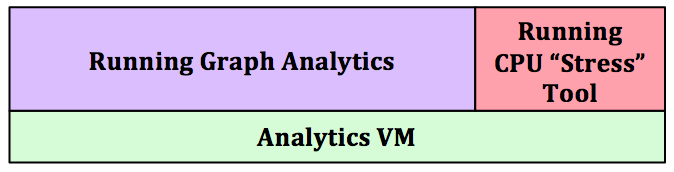
\epsfig{file = figures/RAIDS_testbed_analytics_png, width = 0.5\columnwidth}}
  % \caption{RADS testbed for examining CloudSuite Graph Analytics application behaviour under backdoor channel attack and spike affect}
      \caption{Experimental set-up for Graph Analytics application}
  \label{fig:testbed_analytics}
  \vspace{-0.1cm}
\end{figure}
%\vfill

% EXPERIMENTAL SET UP / TESTBED FOR MEDIA STREAMING
%\vfill
\begin{figure}[!h]
  \vspace{-0.2cm}
  \centering
   {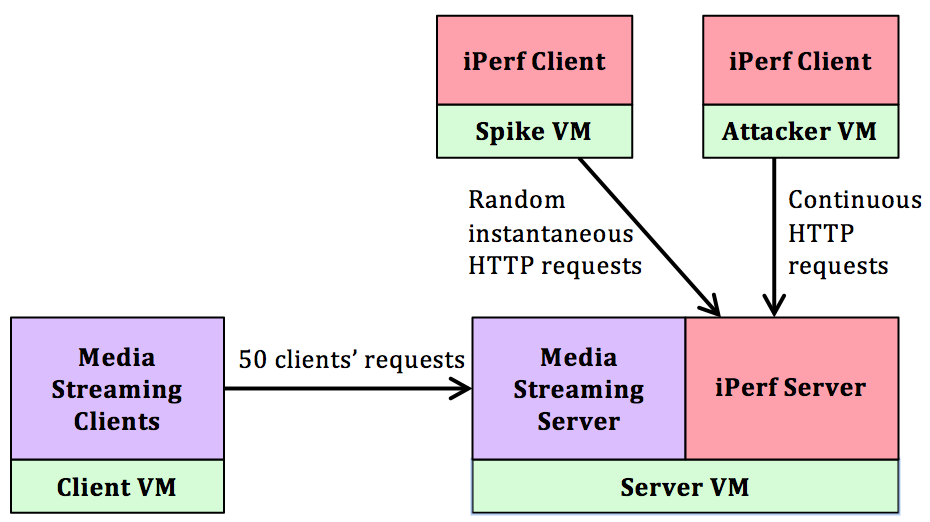
\epsfig{file = figures/RAIDS_testbed_media_png, width = 0.8\columnwidth}}
  % \caption{RAIDS testbed for examining CloudSuite Media Streaming application behaviour under DDoS attack and spike affect}
         \caption{Experimental set-up for Media Streaming application}
  \label{fig:testbed_media}
  \vspace{-0.1cm}
\end{figure}
%\vfill

%\textit{Emulated attacks}: We considered two security attacks in our experiments, which are: backdoor channel attack (for Graph Analytics) and DDoS attack (for Media Streaming). We explained these attacks in detail in Section~\ref{sec:introduction}.
\textit{Emulated attacks}: We emulated the DDoS and the cryptomining attacks targeting the VMs running the Media Streaming server and the Graph Analytics application, respectively. 
%two security attacks in our experiments, which are: backdoor channel attack (for Graph Analytics) and DDoS attack (for Media Streaming). 
Cryptomining attack was emulated by running the ``stress"\footnote{https://people.seas.harvard.edu/\~apw/stress/} tool on the ``Analytics VM" (see Figure~\ref{fig:testbed_analytics}). The ``stress" tool is a simple workload generator, which can impose a configurable amount of CPU, memory, I/O, and disk stress on the system. 
The DDoS attack was emulated by sending continuous HTTP requests from an ``Attacker VM" to the ``Server VM" (see Figure~\ref{fig:testbed_media}) with the help of the iPerf\footnote{https://iperf.fr} tool (``Server VM" as iPerf server and ``Attacker VM" as iPerf client).
%The tool consumes 1/2/3 cores of CPU at different time, which is to produce low-high intensity attacks (low: 1 core, medium: 2 cores, high: 3 cores).
%\todo[author=DSN,inline]{Is this practice of emulating backdoor channel attacks of different intensity by hijacking a different number of cores established? I would think that an attacker would just go for a massive number of VMs (processes, threads,...) to instantiate the attack, without caring too much about how many cores the machine has. Questionmark about methodology here.}
%The DDoS attack is emulated by sending video requests to the Media Streaming server from three different VMs: VM1, VM2, and VM3, which are assumed to be victimised by DDoS attack. Each of these VMs runs 25 clients. They start running the clients at a different time to produce low-high intensity attacks (low: $25$ clients, medium: $25+25$ clients, high: $25+25+25$ clients). 

\textit{Emulated workload spikes}: For the Graph Analytics application, a workload spike was generated by running the ``stress" tool in the ``Analytics VM" for a short period of time (5 seconds). For Media Streaming application, a workload spike was generated by sending HTTP requests for instantaneous period of time (5 seconds) from the ``Attacker VM" to the ``Sever VM" (see Figure~\ref{fig:testbed_media}) with the help of the iPerf tool (``Server VM" as iPerf server and ``Spike VM" as iPerf client).
%\textit{Data Collection}: 
%RAIDS performs both the training of the OCC models and the testing of the test samples for intrusion detection on the hosting node (compute node in case of our test-bed). 
%RADS collected the data required for OCC model training and the anomaly detection by continuously running its \textit{Data Collector} module on the hosting node (compute node in case of our test-bed). 
%RADS \textit{Data Collector} module collected the data required for OCC model training and the anomaly detection by continuously running module on the hosting node (compute node in case of our test-bed). 
%The module stored the data in two different files: (i) \textit{historical\_data\_file}, which stored the historical data required for training and (ii) \textit{current\_data\_file}, which stored the last one minute of data required for testing or anomaly detection. 
%RAIDS \textit{Model Trainer} module performed the training of the OCC models for each Cloud application under examination.  
%RAIDS Training Optimiser algorithm (Algorithm~\ref{raids_algorithm_training_optimiser}) decided the training duration. 
%RAIDS \textit{Intrusion Detector} module tested the test samples and flagged an intrusion whenever it detected an ``anomaly".

%\subsubsection{Experimental Set-up for Offline Experiment}
 %Offline experiments were carried out on the real workload traces [7], which are collected from a Cloud data centre named Bitbrains.

%\subsubsection{Performance Metrics}
\textbf{Performance Metrics:} 
We use a number of standard performance metrics such as precision, recall, accuracy (F1 score), and false positive rate (FPR) to measure the performance of RADS. 
%We use two performance metrics: accuracy (F1 score), and false positive rate (FPR) to measure the performance of RADS. 
%Since RAIDS uses OCC algorithm for identifying the intrusions, all the training data are labelled as "normal". 
RADS reacts with an anomaly alarm whenever it classifies a test sample as ``anomalous", otherwise RADS does not react. 
In our experiments, we declare: (a) False Positives (FP) when RADS raises an alarm but there is no ``anomaly", (b) False Negatives (FN) when RADS fails to raise an alarm but there exists an ``anomaly", (c) True Positives (TP) when RADS raises an alarm and there exists an ``anomaly", (d) True Negatives (TN) when RADS does not raise an alarm and there is no ``anomaly". We define the performance metrics in Equations \ref{eq2}-\ref{eq5}.

% EQUATIONS FOR PERFORMANCE METRICS..
\begin{equation}\label{eq2}
    Precision \quad = \quad   \frac{TP}{TP+FP}
\end{equation}
\begin{equation}\label{eq3}
    Recall \quad = \quad   \frac{TP}{TP+FN}
\end{equation}
\begin{equation}\label{eq4}
    Accuracy (F1 score) \quad = \quad   2\times\frac{Precision \times Recall}{Precision+Recall}
\end{equation}
\begin{equation}\label{eq5}
    FPR \quad = \quad   \frac{FP}{FP+TN}
\end{equation}

Precision gives us the measure of how many of the positive classifications (anomaly alarms) are correct, whereas the recall gives us the measure of RADS's ability to correctly identify an ``anomaly". 
However, precision and recall alone cannot judge the performance of RADS. Therefore, we use Accuracy (F1 score) which gives us the harmonic mean of precision and recall.

%\subsubsection{Training and Testing Data Preparation}
%RAIDS is a real-time IDS where both the training of the classification models and the testing of the new data samples (for intrusion detection) are performed in real-time. RAIDS collected the data for both the training and the testing by continuously running its \textit{data collector} module. The module stored the data in to two different files: (i) \textit{historical\_data\_file}, which stored the historical data required for training and (ii) \textit{current\_data\_file}, which stored the last one minute of data required for testing or intrusion detection. RAIDS training optimiser algorithm decided the amount of historical data required to correctly train the classification models. RAIDS \textit{intrusion detection} module started running only when the classification models were correctly built by RAIDS \textit{model training} module.

% DETECTION RESULTS TABLE

\begin{landscape}

\newcolumntype{L}[1]{>{\raggedright\arraybackslash}p{#1}}
\newcolumntype{C}[1]{>{\centering\arraybackslash}p{#1}}
\newcolumntype{R}[1]{>{\raggedleft\arraybackslash}p{#1}}
\begin{table*}[t]
%\caption{Anomaly detection results of RADS under different data pre-processing approaches}
\caption{Anomaly detection results of RADS under different time series analyses}
\label{tab:test_results} 
\centering
\begin{tabular}{C{2.2cm}C{4.2cm}C{1.7cm}C{1.7cm}C{1.7cm}C{1.5cm}C{1.6cm}} %C{1.5cm}}
  %\hline
  \toprule
  Monitored VM & Time Series Analysis & Training Time (minutes) & \textit{Attack Test} Result & \textit{Spike Test} Result 
  & Accuracy (F1 Score) & False Positive Rate (FPR)\\ %& Overall detection accuracy \\
    \bottomrule
   & & &\begin{tabular}{C{0.5cm}C{0.5cm}}  TP & FN \\  \end{tabular} & \begin{tabular}{C{0.5cm}C{0.5cm}}  FP & TN \\  \end{tabular} \\
    \bottomrule 
        \begin{tabular}{C{2cm}} Graph Analytics VM \\ \end{tabular} 
        & \begin{tabular}{C{4.0cm}} Average \\ Entropy \\ Average \& Std. Deviation \\ \end{tabular} 
        & \begin{tabular}{C{1.2cm}} 45 \\ 105 \\ 130 \end{tabular}
        %& \begin{tabular}{C{1.0cm}} 10 \\  0 \\ 9 \end{tabular}
        %& \begin{tabular}{C{1.0cm}} 10 \\  0 \\ 9 \end{tabular}
         &\begin{tabular}{C{0.5cm}C{0.5cm}} 10 & 0 \\ 0 & 10 \\ 9 & 1 \end{tabular}
         &\begin{tabular}{C{0.5cm}C{0.5cm}} 6 & 24 \\ 2 & 28 \\ 1 & 29 \end{tabular} 
         & \begin{tabular}{C{1.0cm}} 0.77 \\ 0.00 \\ 0.90 \end{tabular}
        & \begin{tabular}{C{1.0cm}} 0.20 \\ 0.07 \\ 0.03 \end{tabular} \\
         %&  \begin{tabular}{C{2.0cm}} 6 \\ 2 \\ 1 \end{tabular} 
         %&  \begin{tabular}{C{2.0cm}} 6 \\ 2 \\ 1 \end{tabular} \\
         

  \hline
    \begin{tabular}{C{2cm}} Media Streaming Server VM \\ \end{tabular} 
       & \begin{tabular}{C{4.0cm}} Average \\ Entropy \\ Average \& Std. Deviation \\  \end{tabular} 
       & \begin{tabular}{C{1.2cm}} 70 \\ 20 \\ 35 \end{tabular}
       %& \begin{tabular}{C{2.0cm}} 10 \\ 10 \\ 9 \end{tabular}
      % & \begin{tabular}{C{2.0cm}} 10 \\ 10 \\ 9 \end{tabular}
      % & \begin{tabular}{C{2.0cm}}  8 \\ 0 \\ 0 \end{tabular}
       &\begin{tabular}{C{0.5cm}C{0.5cm}} 10 & 0 \\ 10 & 0 \\ 9 & 1 \end{tabular}
       &\begin{tabular}{C{0.5cm}C{0.5cm}} 8 & 22 \\ 0 & 30 \\ 0 & 30 \end{tabular} 
        & \begin{tabular}{C{1.0cm}} 0.71 \\ 1.00 \\ 0.95 \end{tabular}
       & \begin{tabular}{C{1.0cm}} 0.27 \\ 0.00 \\ 0.00 \end{tabular} \\
      % & \begin{tabular}{C{2.0cm}}  8 \\ 0 \\ 0 \end{tabular} \\
    \hline
      
\end{tabular}
\end{table*}

\end{landscape}


% END OF DETECTION RESULTS TABLE

%% ACCURACY RESULTS  TABLE
%\newcolumntype{L}[1]{>{\raggedright\arraybackslash}p{#1}}
%\newcolumntype{C}[1]{>{\centering\arraybackslash}p{#1}}
%\newcolumntype{R}[1]{>{\raggedleft\arraybackslash}p{#1}}
%\begin{table*}[t]
%\caption{Effectiveness results of RAIDS under different data pre-processing approaches}
%\label{tab:accuracy_results} 
%\centering
%%\begin{tabular}{|c|c|}
%\begin{tabular}{C{3.0cm}C{4.5cm}C{1.5cm}C{1.5cm}C{1.5cm}C{1.5cm}C{1.7cm}} %C{1.5cm}}
%  \toprule
%  Monitored VM & Data Pre-processing Approach & Number of Observations & Precision & Recall & Accuracy (F1 Score) & False Positive Rate (FPR) \\ %& Overall detection accuracy \\
%    \bottomrule
%        \begin{tabular}{C{2.5cm}} Graph Analytics VM \\ \end{tabular} 
%        & \begin{tabular}{C{4.0cm}} Average \\ Entropy \\ Average \& Standard Deviation \\ \end{tabular} 
%        & \begin{tabular}{C{1.2cm}} 40 \\ 40 \\ 40 \end{tabular} 
%        & \begin{tabular}{C{1.2cm}} 0.63 \\ 0.00 \\ 0.90 \end{tabular}
%         & \begin{tabular}{C{1.2cm}} 1.00 \\ 0.00 \\ 0.90 \end{tabular}
%        & \begin{tabular}{C{1.2cm}} 0.77 \\ 0.00 \\ 0.90 \end{tabular}
%        & \begin{tabular}{C{1.2cm}} 0.20 \\ 0.07 \\ 0.03 \end{tabular} \\
%       
%  \hline
%    \begin{tabular}{C{2.5cm}} Media Streaming Server VM \\ \end{tabular} 
%       & \begin{tabular}{C{4.0cm}} Average \\ Entropy \\ Average \& Standard Deviation \\ \end{tabular} 
%       & \begin{tabular}{C{1.2cm}} 40 \\ 40 \\ 40 \end{tabular}
%       & \begin{tabular}{C{1.2cm}} 0.56 \\ 1.00 \\ 1.00 \end{tabular}
%       & \begin{tabular}{C{1.2cm}} 1.00 \\ 1.00 \\ 0.90 \end{tabular}
%       & \begin{tabular}{C{1.2cm}} 0.71 \\ 1.00 \\ 0.95 \end{tabular}
%       & \begin{tabular}{C{1.2cm}} 0.27 \\ 0.00 \\ 0.00 \end{tabular} \\
%
%    \hline
%      
%\end{tabular}
%\end{table*}
%
% END OF ACCURACY RESULTS TABLE

%\subsubsection{\textbf{Anomaly Detection Performance of RADS}}
\textbf{Anomaly Detection Performance of RADS:}
%To evaluate the anomaly detection performance of RADS we carried out two tests: (i) \textit{Attack Test} which analyses the number of successful anomaly detections by RADS and (ii) \textit{Spike Test} which analyses the number of false positives generated by RADS. 
To evaluate the anomaly detection performance of RADS we carried out two tests: (i) \textit{Attack Test -} during which we emulated the DDoS attack (targeting the VM running the Media Streaming server) or the cryptomining attack (targeting the VM running the Graph Analytics application) continuously for 10 minutes; and (ii) \textit{Spike Test -} during which we emulated workload spikes for 10 times in a random manner in a time period of 30 minutes; there is no emulated attack during this test.
%To measure the accuracy of RAIDS we performed two tests: (i) \textit{intrusion detection test:} to understand RAIDS's successfulness in detecting Cloud security attacks and (ii) \textit{false positive test:} to understand RAIDS's sensitivity towards normal application behaviour. Table~\ref{tab:detection_results} presents the \textit{intrusion detection test} result which shows the number of successful detections by RAIDS, whereas Table~\ref{tab:false_positives} presents \textit{false positive test} result which show the number of false positives generated by RAIDS. The result for the former test is presented for different attack categories under different data pre-processing approaches, similarly the result for the latter test is presented for different spike categories under different data-processing approaches.
During both the tests, we executed the RADS \textit{Anomaly Detector} module on the hosting node. 
%\textit{Model Trainer} and \textit{Anomaly Detector} module 
For both the tests, the module used the same OCC models which were trained by the RADS \textit{Model Trainer} module. 
%Hence, the training times required for different data pre-processing approaches are the same in both the tests. However, the training time is different for different approaches and for different VMs as it is decided by the RADS \textit{Training Optimiser Algorithm} (Algorithm~\ref{raids_algorithm_training_optimiser}).
%During both the tests, we executed RADS \textit{Anomaly Detector} module 
%Both the testing started only after the OCC models were correctly built by RAIDS \textit{Model Trainer} module. 
%The testing time for \textit{Intrusion Detection Test} was 10 minutes, during which we executed each emulated security attack continuously for 10 minutes, whereas the testing time for the \textit{False Positive Test} was 30 minutes, during which we injected the emulated workload spikes for 10 times in random manner. 
%Table~\ref{tab:attack_spike_category} describes both the attack and the spike categories for both cloud applications. 

Table~\ref{tab:test_results} presents the test results under different time series analyses.
From the results we observe 
%the following:
%\begin{enumerate}[{(a)}]
%\item 
that the average based analysis achieves the maximum number of true positives (total 20), but on the other hand, this approach raises the maximum number of false positives (total 14).
%\item 
Entropy raises only 2 false positives in the case of the Graph Analytics VM and no false positives in the case of the Media Streaming server VM, but the problem with the entropy based approach is its poor performance in detecting the attacks (10 false negatives in the case of the Graph Analytics VM).
%\item 
%The proposed data pre-processing approach which uses a combination of the average and the standard deviation, successfully detects the attacks with total 18 true positives. 
RADS window-based time series analysis, which uses a combination of the average and the standard deviation, successfully detects the attacks with total 18 true positives. 
%, which is however less than the average based approach. We have observed that 
We have observed that the false negatives (1 for each of the monitored VMs) arise during the first minute of the \textit{Attack Test}, when the ``anomalous" behaviour due to attack does not occupy the whole 1 minute of the detection window; the time series of the detection window becomes similar to the one depicted in Figure~\ref{fig:one_minute_timeseries}. A test sample generated from such a detection window can be represented as: (high\_average, high\_standard\_deviation), which is wrongly classified as ``normal" by RADS as it considers the short-term ``anomalous" behaviour in the detection window as a genuine workload spike.
%As these false negatives appear only during the first minute of the attack, 
However, these false negatives are trivial due to the fact that they appear only during the first minute of the attack; and DDoS or cryptomining attacks require a considerable amount of time (at least a few minutes) before they become harmful.  
%However, such false negatives do not affect DDoS or cryptomining attack detection as these kind of attacks persist for a long period of time (at least longer than 1 minute) to achieve their goals.
%\item The proposed data pre-processing approach which uses a combination of the average and the standard deviation achieves a good success rate (90\%) in detecting the attacks, which is however less than the average based approach. We have observed that the single time failure of the proposed approach occurs for the first instance of the detection process. During the first minute of the detection process, when the ``anomalous" behaviour due to attack does not occupy the whole 1 minute of the detection window, the timeseries of the detection window becomes similar to the one depicted in Figure~\ref{fig:one_minute_timeseries}. A test sample generated from such a detection window can be represented as: (high\_average, high\_standard\_deviation), which is wrongly classified as ``normal" by RAIDS as it considers that there are genuine workload spikes in the detection window. 
% as a result of obeying the \textbf{assumption} (made in Section~\ref{sec:approach}): \textit{genuine workload spikes during a Cloud application's normal behaviour produce high average values, which are accompanied by very high standard deviation values.}
%We consider the solution of this as future work.
%\end{enumerate}

% ONE MINUTE TIMESERIES
%\vfill
\begin{figure}[!h]
%  \vspace{-0.2cm}
  \centering
      {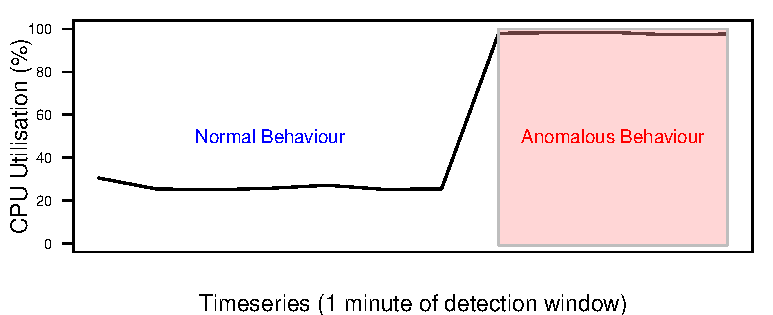
\epsfig{file = figures/one_minute_timeseries, width = 0.8\columnwidth}}
   \caption{The first minute of detection window which includes both the ``normal" and the ``anomalous" behaviour}
  \label{fig:one_minute_timeseries}
 % \vspace{-0.1cm}
\end{figure}
%\vfill

%Therefore, RAIDS wrongly identifies this high value of standard deviation due to security attack as a normal behaviour occurring due to spikes. However, the impact of this depends on the behaviour of the security attack; if the attack establishes gradually i.e. step by step without jumping to high intensity attack straight away, we can expect RAIDS to be able to detect even the first time occurrence of the attack. In any case, we consider this issue to analyse and diagnose further in future.  
		%\todo[author=DSN,inline]{Can you back this argument up with a citation or more experimental evidence?}
%Table~\ref{tab:test_results} further presents the accuracy (F1 score) and the false positive rate (FPR) results of RAIDS under different data pre-processing approaches. In the Table~\ref{tab:accuracy_results}, the number of observations are calculated by adding the number of testing samples in \textit{Intrusion Detection Test} and \textit{False Positive Test}, i.e. ($10+30=40$). All the performance metrics are calculated based on the ``number of successful detections'' and ``false positives'' observed from the two tests (Table~\ref{tab:test_results}).
In order to get a better insight into the anomaly detection performance of RADS, we calculated the accuracy (F1 score) and the false positive rate (FPR) (see Table~\ref{tab:test_results}) using Equations \ref{eq4} and \ref{eq5}, respectively.  
%From the results presented in Table~\ref{tab:accuracy_results} we answer the research question 1 as follows:
These performance metrics answer the research questions 1 and 2 as follows:
\begin{enumerate}[{(a)}]
\item RADS can detect Cloud anomalies occurring due to DDoS and cryptomining attacks in real-time with an accuracy (F1 Score) of 90-95\% and a low false positive rate of 0-3\%.
\item RADS achieves on average 34\% improvement in accuracy and 60\% improvement in false positive rate while using its window-based time series analysis instead of using the state-of-the-art average or entropy based analysis. 
% (based on average and entropy).
%\item Results show that RAIDS achieves 90-95\% accuracy (F1 score) with a low false positive rate of 0-3\% while using the proposed data pre-processing approach which uses the combination of both the average and the standard deviation.
%\item The results further reveal on average 34\% improvement in accuracy and 60\% improvement in false positive rate while using the proposed data pre-processing approach instead of using the state-of-the-art data pre-processing approaches for Cloud IDSs which are based on either the average or the entropy.
%\item Accuracy (F1 score) results show that RAIDS achieves 87-95\% accuracy with a low false positive rate of 0-3\% using its unique data pre-processing approach that uses combination of both the average and the standard deviation.
%\item Accuracy (F1 score) results demonstrate that RAIDS achieves on average 88\% improvement in accuracy and 35\% improvement in false positive rates while using its unique data pre-processing approach instead of using state-of-the-art average or entropy based approaches.
\end{enumerate}
%The anomaly detection performance achieved by RADS in our experiments may vary under different experimental set-up. The performance results discussed above are only indicators of RADS capability in detecting DDoS and cryptomining attacks with high accuracy and low false positive rates.

%\subsubsection{\textbf{Efficiency of RADS}}
\textbf{Efficiency of RADS:}
%In this section we evaluate the efficiency of RAIDS. 
%RAIDS is a real-time IDS and therefore, its important for RAIDS to be efficient in terms of the hosting node resource that it consumes and the time it takes while performing the training of the classification models and the testing of the new samples to detect the intrusions. 
%To evaluate the efficiency of RAIDS we carried out two experiments: (i) \textit{Training Efficiency} which measures the efficiency of RAIDS in training OCC models and (ii) \textit{Testing Efficiency} which measures the efficiency of RAIDS in intrusion detection or testing of the new samples. We performed the experiments on one of the compute nodes in our testbed. 
%The hosting node is a Dell PowerEdge R420 server which runs CentOS 6.6 and has 24 cores, 2-way hyper-threaded, clocked at 2.20 GHz with 24GB DRAM clocked at 1600 MHz. 
%In order to explain the effect of number of hosted VMs on RAIDS efficiency, we carried out the experiments while scaling up the number of VMs from 2 to 10 in the compute node. Although such scaling of VMs does not represent a real Cloud data centre, we attempt to extract out some information on RAIDS efficiency under VM scaled up situations. 
%Also, important to note that, for experimental purpose, we stopped RAIDS \textit{Training Optimiser Algorithm} and considered a fixed number of training data samples for each of the \textit{Training Efficiency} experiments, which ranges from 5 minutes to 25 minutes of data. The data samples for \textit{Testing Efficiency} experiments contain only last 1 minute of data. 
%In order to address the issues of variability, in \textit{training efficiency} experiment, we considered the average measurements from 5 training runs, whereas, in \textit{testing efficiency} experiment, we considered the average measurements from 10 testing runs. 
%We evaluate the efficiency results in terms of overhead on the compute node resources and the time taken to perform the training and the testing. We discuss the results in the following sub-sections.
%In particular, in this section we attempt to answer the research question 4.
To evaluate the efficiency of RADS we carried out experiments while scaling up the number of hosted VMs from 2 to 10. Although such scaling of VMs does not represent a real Cloud data centre, we attempt to extract some information on RADS efficiency under VM scaled up situations. 

% OVERHEAD ON CPU
%\vfill
\begin{figure}[!h]
  \vspace{-0.2cm}
  \centering
   {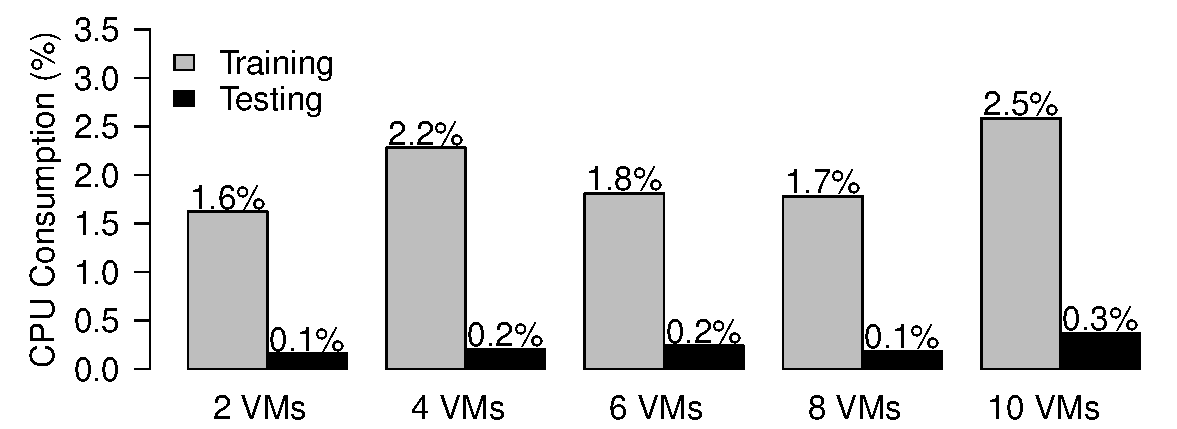
\epsfig{file = figures/overhead_cpu, width = 0.8\columnwidth}}
   \caption{Hosting node CPU consumption by RADS}
  \label{fig:overhead_cpu}
  \vspace{-0.1cm}
\end{figure}
%\vfill

% RAIDS TRAINING AND TESTING TIME
%\vfill
\begin{figure}[!h]
  \vspace{-0.2cm}
  \centering
   {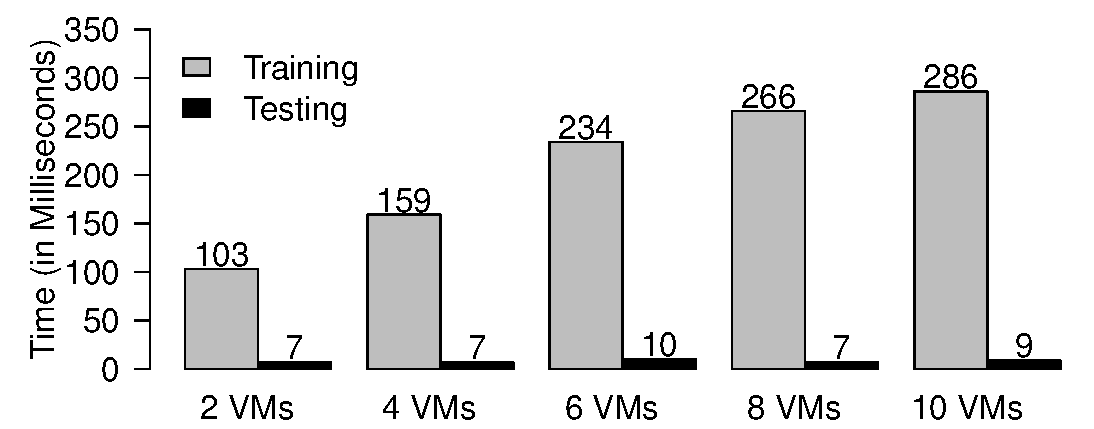
\epsfig{file = figures/overhead_time, width = 0.8\columnwidth}}
   \caption{Training and testing time required by RADS}
  \label{fig:overhead_time}
  \vspace{-0.1cm}
\end{figure}
%\vfill

\textit{Computation cost of RADS:} We measured the computation cost of RADS in terms of its CPU consumption on the hosting node. 
The bar plots in Figure~\ref{fig:overhead_cpu} show the CPU consumed by RADS while performing the training and the testing (anomaly detection).
From the plots we find that for training, the CPU consumption remains very low (in the range 1.6\% to 2.5\%) and it does not increase much with the scaling up of the number of VMs, whereas for testing, the CPU consumption remains consistently negligible. 
%We further found that for data collection, RAIDS consumed a very negligible amount of CPU (around 0.02\%).

\textit{Processing time of RADS}: The bar plots in Figure~\ref{fig:overhead_time} show the processing time that RADS took while performing the training and the testing. From the plots we observe that RADS took milliseconds in finishing the training and the testing tasks. The testing time is much lower than the training time. 
The training time increases with the scaling up of the number of VMs, but the testing time remains almost constant. 

In answering the research question 3, we can summarise that RADS can be used as a lightweight tool in terms of consuming minimal hosting node CPU and processing time in a Cloud data centre. However, the processing time required for training increases with the scaling up of the number of hosted VMs. This may lead to a RADS efficiency issue in the case where there are hundreds or thousands of hosted VMs and when the duration of the training increases to few hours or days. In future, we will attempt to explore this issue and address it with shared-memory or multithreaded programming solutions such as OpenMP, MPI, Phoenix++, etc.
%
%In answering the research question 3, we summarise the above observations as follows:
%\begin{enumerate}[{(a)}]
%\item RADS consumes minimal hosting node CPU during both training and testing. RADS can maintain its efficiency in terms of its CPU consumption even when there is scaling up of the number of hosted VMs.
%\item RADS processing time is minimal, however, the time required for training increases with the scaling up of the number of hosted VMs. This may lead to RADS efficiency issue in case when there are hundreds and thousands of hosted VMs and when the number of training data samples increase to few hours or days. 
%%However, the impact of such an issue should not persist long due to the fact that the training for a particular cloud application behaviour runs every 5 minutes and it stops when the RAIDS training optimiser algorithm (discussed in Section~\ref{sec:algorithm}) decides that the OCC model for that application is correctly built. Nevertheless, 
%In future, we will attempt to explore this issue and address it with shared-memory or multithreaded programming solutions such as OpenMP, MPI, Phoenix++ etc.
%\end{enumerate}

%\subsection{Evaluation of RAIDS Using Real-world Cloud Workload Trace}
\subsection{Real-world Experiments}
\label{sec:offline_analysis}
%In this section we evaluate the performance of RADS in terms of dealing with the genuine workload spikes observed in the real-world Cloud data centre workload trace. 
\noindent In this section we evaluate the performance of RADS in terms of false positive rate by analysing real-world Cloud workload traces. Specifically, in this section we attempt to answer research question 4.

%\subsubsection{Real-world Cloud Workload Trace Description}
%There are studies of Cloud workload traces such as~\cite{azure:2017}, \cite{Google:2012}, \cite{IBM:2014}, \cite{yahoo:2011}, \cite{FB:2012} which analysed the online traces collected from giant datacenter operators such as Microsoft, Google, IBM, Yahoo, Facebook etc. These traces do not represent Cloud data centre workloads in general; rather they represent workloads which may be typical for operations specific to these companies. Moreover, these studies do not include information regarding network traffic of the VMs, which is one of the metrics that we consider in RAIDS. 
%Therefore, as the real-world Cloud workload trace we used the traces from~\cite{workloadCCGRID:2015}. These traces are collected from a Cloud data centre named Bitbrains\footnote{https://www.solvinity.com}, which specialises in managed hosting and business computation for enterprises such as banks, credit card operators, insurers etc. Thus, the traces represent business critical workloads which generally use the same VM for long period of time. This is an important aspect for evaluating RAIDS performance as RAIDS assumes that for each VM, the application running during the testing period is the same application that was running during the training period. 
%The traces contain seven performance metrics including CPU utilisation and network throughput of 1,750 VMs from Bitbrains. The metrics are sampled every 5 minute. The traces were collected between July and September 2013 in two trace directories: (i) \textit{fastStorage} which consists of 1,250 VMs that are connected to fast storage area network (SAN) storage devices and (ii) \textit{Rnd} which consists of 500 VMs that are either connected to the fast SAN devices or to much slower Network Attached Storage (NAS) devices. \textit{fastStorage} contains one months of trace (August, 2013), whereas \textit{Rnd} contains three months of trace (July-September, 2013).
%\subsubsection{Real-world Cloud Workload Trace Description}
%\subsubsection{Trace Description}
\textbf{Trace Description:}
%RADS uses application-specific behavioural models to detect behavioural anomalies inside the VMs occurring due to security attacks. 
%Therefore, RAIDS can achieve maximum accuracy only when the VMs run the same Cloud application or workload throughout the training and the testing/detection phase. In order to obtain traces collected from VMs running the same Cloud application throughout the trace collection period, we carried out an investigation on available real-world Cloud workload traces. 
%In order to obtain the real-world Cloud workload traces, we carried out an investigation on available real-world Cloud workload traces. 
We selected the traces collected from a Cloud data centre named Bitbrains\footnote{https://www.solvinity.com} as analysed in~\cite{workloadCCGRID:2015}. % to use them as the real-world Cloud workload trace. 
Bitbrains specialises in managed hosting and business computation for enterprises such as banks, credit card operators, insurers, etc. 
%Researchers in~\cite{azure:2017, Google:2012, IBM:2014, yahoo:2011, FB:2012} analysed the real-world Cloud workload traces collected from giant datacenter operators such as Microsoft, Google, IBM, Yahoo, Facebook etc. These traces do not represent Cloud data centre workloads in general; rather they represent workloads which may be typical for operations specific to these companies. Moreover, these studies do not include information regarding network traffic of the VMs, which is one of the metrics that we consider in RADS. 
%The work in~\cite{workloadCCGRID:2015} analysed the traces collected from a Cloud data centre named Bitbrains\footnote{https://www.solvinity.com}, which specialises in managed hosting and business computation for enterprises such as banks, credit card operators, insurers etc. 
%Thus, these traces represent business critical workloads which generally use the same VM for long periods of time. 
%Based on our investigation, we selected the traces collected from Bitbrains as analysed in~\cite{workloadCCGRID:2015} to use them as the real-world Cloud workload trace. 
%These traces were collected from a Cloud data centre named Bitbrains\footnote{https://www.solvinity.com}, which specialises in managed hosting and business computation for enterprises such as banks, credit card operators, insurers etc. Thus, the traces represent business critical workloads which generally use the same VM for long period of time. 
%This is an important aspect for evaluating RAIDS performance as RAIDS assumes that for each VM, the application running during the testing period is the same application that was running during the training period. 
The traces contain seven performance metrics including CPU utilisation and network throughput of 1,750 VMs. The metrics are sampled every 5 minutes. The traces were collected between July and September 2013 in two trace directories: (i) \textit{fastStorage} which consists of 1,250 VMs that are connected to fast storage area network (SAN) storage devices and (ii) \textit{Rnd} which consists of 500 VMs that are either connected to the fast SAN devices or to much slower Network Attached Storage (NAS) devices. \textit{fastStorage} contains one month of trace (August, 2013), whereas \textit{Rnd} contains three months of trace (July-September, 2013).
%As we had limited knowledge of these traces, we could not choose the VMs which run the same application consistently throughout the data collection period. However, 
%We selected three consecutive days of traces to make an assumption that the Cloud applications or workloads running inside the VMs are consistent throughout the experimental period. 
%Therefore, RAIDS is designed for detecting security attacks on VMs which run the same Cloud application continuously throughout the training and the testing phase of RAIDS. 
 %that for each VM, the application running during the testing period is the same application that was running during the training period. 
%There are studies of Cloud workload traces such as~\cite{azure:2017}, \cite{Google:2012}, \cite{IBM:2014}, \cite{yahoo:2011}, \cite{FB:2012} which analysed the online traces collected from giant datacenter operators such as Microsoft, Google, IBM, Yahoo, Facebook etc. These traces do not represent Cloud data centre workloads in general; rather they represent workloads which may be typical for operations specific to these companies. Moreover, these studies do not include information regarding network traffic of the VMs, which is one of the metrics that we consider in RAIDS. 
%Therefore, as the real-world Cloud workload trace we collected the traces from~\cite{workloadCCGRID:2015}. These traces are collected from a Cloud data centre named Bitbrains\footnote{https://www.solvinity.com}, which specialises in managed hosting and business computation for enterprises such as banks, credit card operators, insurers etc. Thus, the traces represent business critical workloads which generally use the same VM for long period of time. 
%%This is an important aspect for evaluating RAIDS performance as RAIDS assumes that for each VM, the application running during the testing period is the same application that was running during the training period. 
%The traces contain seven performance metrics including CPU utilisation and network throughput of 1,750 VMs from Bitbrains. The metrics are sampled every 5 minute. The traces were collected between July and September 2013 in two trace directories: (i) \textit{fastStorage} which consists of 1,250 VMs that are connected to fast storage area network (SAN) storage devices and (ii) \textit{Rnd} which consists of 500 VMs that are either connected to the fast SAN devices or to much slower Network Attached Storage (NAS) devices. \textit{fastStorage} contains one months of trace (August, 2013), whereas \textit{Rnd} contains three months of trace (July-September, 2013).

%\subsubsection{Preparation of Traces}
\textbf{Preparation of Traces:}
\label{sec:preparaiton_of_traces}
In order to use the traces from~\cite{workloadCCGRID:2015} for evaluating the performance of RADS, we made the following selection process:
\begin{enumerate}[{(1)}]
\item We selected only the traces from the month August, 2013 for which both the traces (\textit{fastStorage} and \textit{Rnd}) were available. 
\item We further selected the first three days of traces, making the assumption that the Cloud applications or workloads running inside the VMs are consistent throughout the experimental period. 
%\item We further selected only the first three days of traces for ease of experiment. 
%\item We further selected only the first three days of traces so that we can make the following assumption: \textit{throughput the lifetime of the trace collection each monitored VM executed only a single application and that application continued to run in the same VM.}
\item Out of the three days of traces, we selected the first two days (14:40, 12 August to 14:40, 14 August 2013) of traces for training and and the third day (14:40, 14 August to 14:40, 15 August 2013) of traces for testing. 
\item We performed spike detection analysis on the traces using the Interquartile Range (IQR\footnote{https://en.wikipedia.org/wiki/Interquartile\_range}) algorithm and selected traces only from VMs which flagged spikes. This is because we intend to evaluate the performance of RADS in terms of dealing with the genuine workload spikes observed in the traces. 
\item Finally, for CPU utilisation analysis, we selected traces from VMs which have CPU utilisation greater than 10\%, and for network throughput analysis we selected the traces from VMs with network throughput greater than 100KB/s. This is done in order to select traces from active VMs which are running a decent amount of workload. 
%Thus, we selected the traces from 82 VMs for CPU utilisation analysis and 212 VMs for network throughput analysis. 
\end{enumerate}

Following the above selection process, we chose the traces from 82 VMs for CPU utilisation analysis and traces from 212 VMs for network throughput analysis.

% OFFLINE  TIMESERIES GRAPHS
%\vfill
\begin{figure}[!h]
  %\vspace{-0.2cm}
  \centering
   {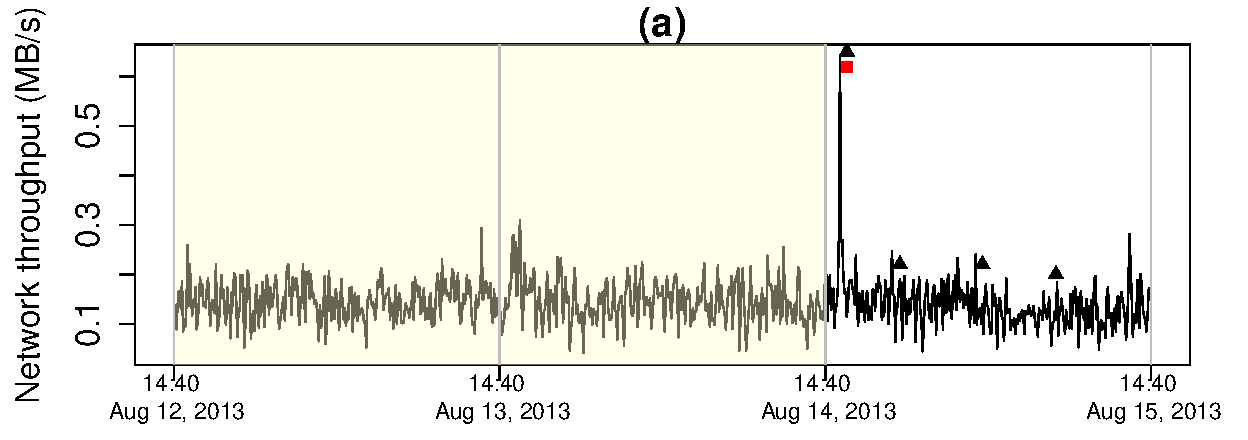
\epsfig{file = figures/realworld_network_941, width = 0.8\columnwidth}}
    {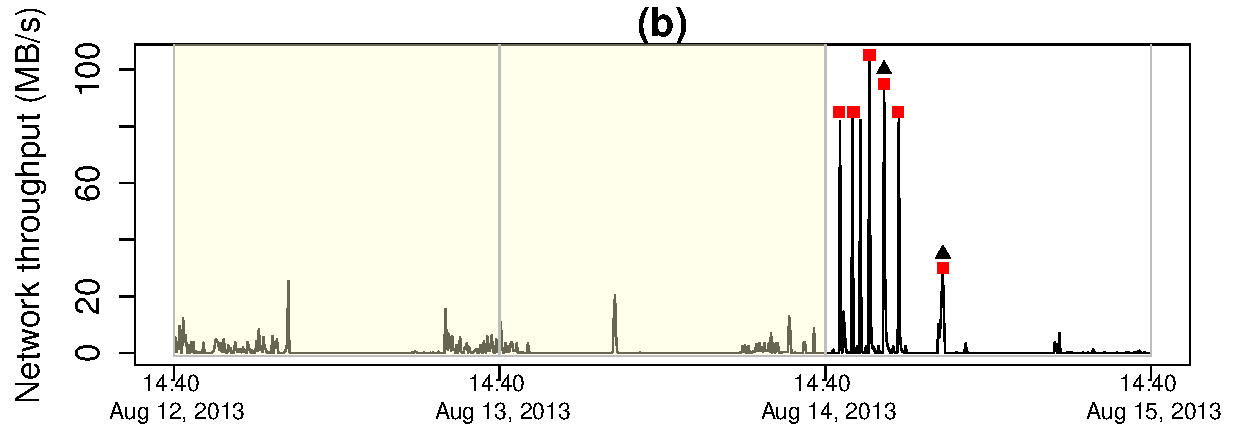
\epsfig{file = figures/realworld_network_357, width = 0.8\columnwidth}}
      {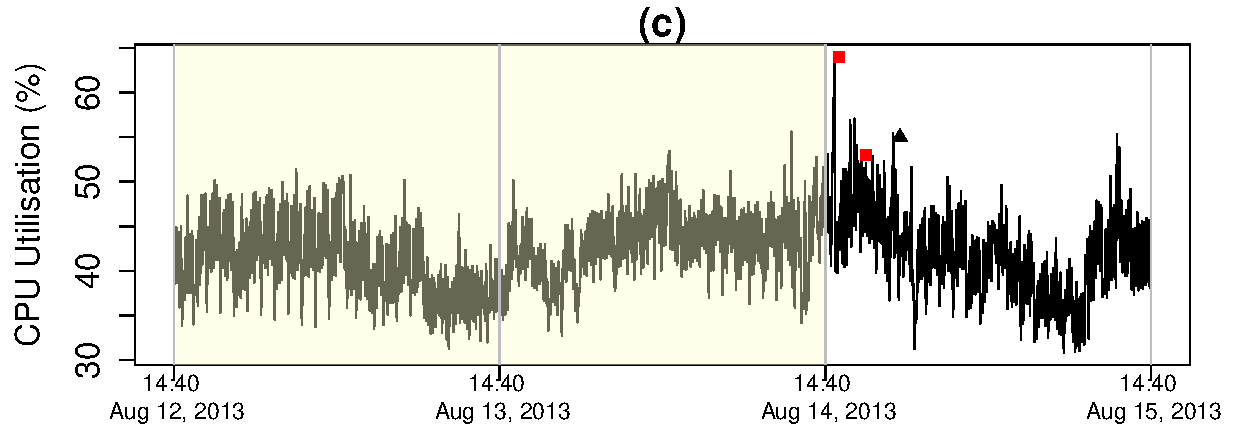
\epsfig{file = figures/realworld_cpu_980, width = 0.8\columnwidth}}
         {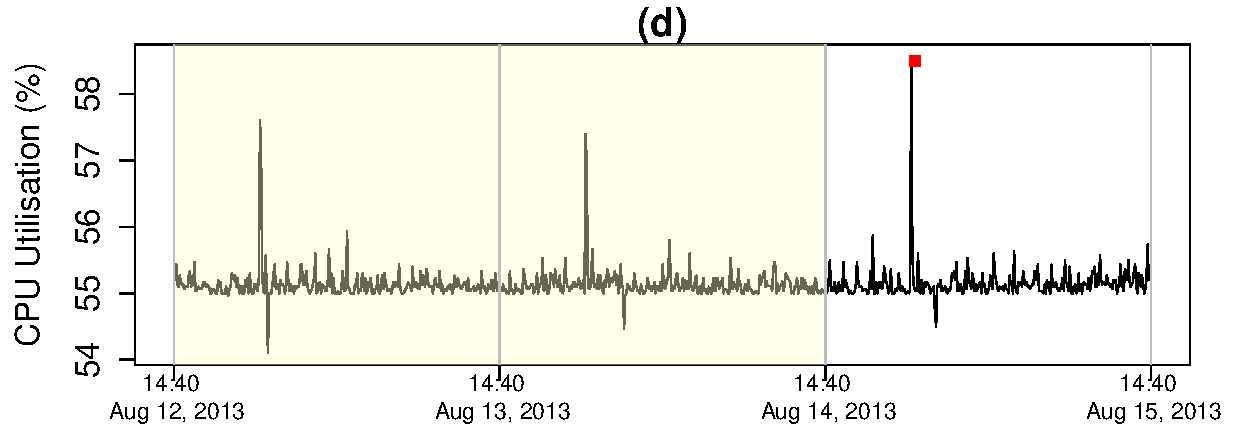
\epsfig{file = figures/realworld_cpu_1556, width = 0.8\columnwidth}}
           % {\epsfig{file = figures/realworld_network_1025, width = \columnwidth}}
  % \caption{Performance of RAIDS on different VM traces collected from the Grid Workload Archives [ref]: (a) VM-941 from fastStorage trace, (b) VM-357 from fastStorage trace, (c) VM-980 from fastStorage trace, (d) VM-306 from Rnd trace, (e) VM-1025 from fastStorage trace. The yellow coloured section represent the training period and the section without colour represents the testing period. The coloured shapes represent false alarms while using different data pre-processing approaches by RAIDS: blue round, red square, and black triangle are for average and standard deviation based approach, average based approach, and entropy based approach respectively. }
%      \caption{Responses from RAIDS on different Cloud workload behaviour observed in the traces collected from~\cite{workloadCCGRID:2015}: (a) VM-941 from fastStorage trace, (b) VM-357 from fastStorage trace, (c) VM-980 from fastStorage trace, (d) VM-306 from Rnd trace, (e) VM-1025 from fastStorage trace. The yellow coloured sections represent the training period and the section without colour represents the testing period. The coloured shapes represent ``anomaly" alarms raised by RAIDS while using different data pre-processing approaches: blue round, red square, and black triangle are for proposed approach (average and standard deviation based approach), average based approach, and entropy based approach, respectively. }
      
          % \caption{Responses from RADS on different Cloud workload behaviour observed in the traces collected from~\cite{workloadCCGRID:2015}: (a) VM-941 from fastStorage trace, (b) VM-357 from fastStorage trace, (c) VM-980 from fastStorage trace, (d) VM-306 from Rnd trace. The yellow coloured sections represent the training period and the section without colour represents the testing period. The coloured shapes represent ``anomaly" alarms raised by RADS while using different data pre-processing approaches: red square and black triangle are for the average and the entropy based approaches, respectively. }
           
                      \caption{RADS analysis of different Cloud workload behaviour observed in the traces collected from~\cite{workloadCCGRID:2015}: (a) VM-941 from fastStorage trace, (b) VM-357 from fastStorage trace, (c) VM-980 from fastStorage trace, (d) VM-306 from Rnd trace. The yellow coloured section represents the training period and the section without colour represents the testing period. The coloured shapes represent ``anomaly" alarms raised by RADS while using different time series analyses: red square and black triangle are for the average and the entropy based analysis, respectively. }



  \label{fig:offline_timeseries}
  %\vspace{-0.1cm}
\end{figure}
%\vfill


%\subsubsection{Performance of RADS Under Different Cloud Workload}
\textbf{Performance of RADS Under Different Cloud Workloads:}
%Out of the selected traces, we chose the traces from certain VMs, which experience different workload behaviour as presented in Figure~\ref{fig:offline_timeseries} using the timeseries graphs.
%In the figure, the left two yellow coloured sections represent the training period trace with which we trained the RAIDS classifier, whereas the right section without any colour represent the testing period trace for which we observe the responses from RAIDS. 
%\begin{enumerate}[{(a)}]
%\item \textit{VM-941 from fastStorage trace}: Figure~\ref{fig:offline_timeseries}(a) shows the network throughput for VM-941 collected from \textit{fastStorage} trace. From the figure we observe that the network throughput for this VM is consistently fluctuating throughput the training and the testing period and there is one significant genuine workload spike occurring during the testing period. 
%\item \textit{VM-357 from fastStorage trace} (Figure~\ref{fig:offline_timeseries}(b)): Figure~\ref{fig:offline_timeseries}(b) shows the network throughput for VM-357 collected from \textit{fastStorage} trace. 
%From the figure we observe that the network throughput for this VM is irregularly fluctuating throughput the training and the testing period and there are multiple significant genuine workload spikes occurring during the testing period.
%\item \textit{VM-980 from fastStorage trace} (Figure~\ref{fig:offline_timeseries}(c)): consistently fluctuating CPU utilisation behaviour during both the training and the testing period. Multiple insignificant genuine workload spike occurring during the testing period. 
%\item \textit{VM-306 from Rnd trace} (Figure~\ref{fig:offline_timeseries}(d)): consistently fluctuating CPU utilisation behaviour during both the training and the testing period. Insignificant genuine workload spike occurring during the both the training and the testing period. 
%\item \textit{VM-1025 from fastStorage} (Figure~\ref{fig:offline_timeseries}(e)):  irregularly fluctuating network behaviour during the training period. Multiple genuine behavioural change during the testing period with occasional genuine workload spikes.  
%\end{enumerate}
Out of the selected traces, we chose the traces from a range of VMs exhibiting varying workload behaviour as presented in Figure~\ref{fig:offline_timeseries} using the time series graphs. 
%The timeseries graphs reveal how RAIDS responses towards these workload behaviour while using different data pre-processing approaches. We summarise the observations from these graphs as follows.}
The time series graphs reveal how RADS performs under different Cloud workload behaviour while using different time series analyses. We summarise the observations from these graphs as follows:

\begin{enumerate}[{(a)}]
\item In both cases where the workload experiences consistently fluctuating behaviour (Figure~\ref{fig:offline_timeseries}(a)) and irregular behaviour (Figure~\ref{fig:offline_timeseries}(c)), RADS successfully classifies the genuine workload spikes as ``normal" while using its window-based time series analysis. But, while using the average or the entropy based analysis, RADS fails to classify the genuine workload spikes as ``normal" and raises false ``anomaly" alarms. %In fact using the entropy based approach raises three more false alarms. 
\item In both the cases where the workload experiences significant genuine workload spikes (Figures~\ref{fig:offline_timeseries}(a) and (b)) and insignificant genuine workload spikes (Figure~\ref{fig:offline_timeseries}(c)), RADS successfully classifies them as ``normal" while using its window-based time series analysis.  But, while using the average or the entropy based analysis RADS fails to classify them as ``normal" and raises false ``anomaly" alarms.
\item While using its window-based time series analysis, RADS continues its successful classification of genuine workload spikes as ``normal" even when the workload experiences genuine workload spikes during the training period (Figure~\ref{fig:offline_timeseries}(d)). However, using the average based analysis RADS fails again to classify the genuine workload spikes as ``normal" and raises false ``anomaly" alarm. 
%\item During the testing period, when the workload experiences significant behavioural change, which persist for a relatively long period of time (Figure~\ref{fig:offline_timeseries}(e)), RADS can successfully classify that change and raise ``anomaly" alarms while using all the data pre-processing approaches that we consider. 
%This gives us the indication that using the proposed data pre-processing approach, RADS can not only deal with the genuine workload spikes (which persist only for a momentary period of time) but also it can successfully detect the ``anomalies" occurring due to the cybersecurity attacks (which persist for a relatively long period of time).
%\item When the workload experiences significant and consistent behavioural change during the testing period (Figure~\ref{fig:offline_timeseries}(e)), RAIDS can successfully classify that change and raise ``anomaly" alarms while using all the data pre-processing approaches that we consider. 
%\textcolor{blue}{This gives us the indication that using the proposed data pre-processing approach, RAIDS can not only deal with the genuine workload spikes but also it can successfully detect the ``anomalies" occurring due to the security attacks. This is because genuine workload spikes are differentiated from the security attacks by considering the fact that spikes persist only for a momentary period of time, whereas security attacks persist for a relatively long period of time.}
\end{enumerate}

% RAIDS VERSIONS  TABLE
%\newcolumntype{L}[1]{>{\raggedright\arraybackslash}p{#1}}
%\newcolumntype{C}[1]{>{\centering\arraybackslash}p{#1}}
%\newcolumntype{R}[1]{>{\raggedleft\arraybackslash}p{#1}}
%\begin{table}[t]
%%\caption{Different versions of RAIDS using different data pre-processing approaches and different number of artificial data points}
%\caption{Different experiments performed for RADS}\
%%\caption{Experiment details}
%\label{tab:raids_versions} 
%\centering
%%\begin{tabular}{|c|c|}
%\begin{tabular}{C{1cm}C{4cm}C{2.8cm}} %C{1.5cm}}
%  \toprule
%   Experiment & Data Pre-processing Approach & Artificial Data Points \\ %& Overall detection accuracy \\
%    \bottomrule
%        \begin{tabular}{C{0.7cm}} RADS1 \\ RADS2 \\ RADS3 \\ AVG \\ ENT \\  \end{tabular} 
%        & \begin{tabular}{C{3.7cm}} Average \& Standard Deviation \\ Average \& Standard Deviation \\ Average \& Standard Deviation \\ Average \\ Entropy \end{tabular} 
%        & \begin{tabular}{C{2.7cm}}  1x of raw data points \\  2x of raw data points \\  3x of raw data points \\ No artificial data points \\ No artificial data points \end{tabular} \\
%       
%    \hline
%      
%\end{tabular}
%\end{table}

% END OF RAIDS VERSIONS  TABLE

% OFFLINE CPU AND NETWORK ANALYSIS
%\vfill
\begin{figure}[!h]
%  \vspace{-0.2cm}
  \centering
   {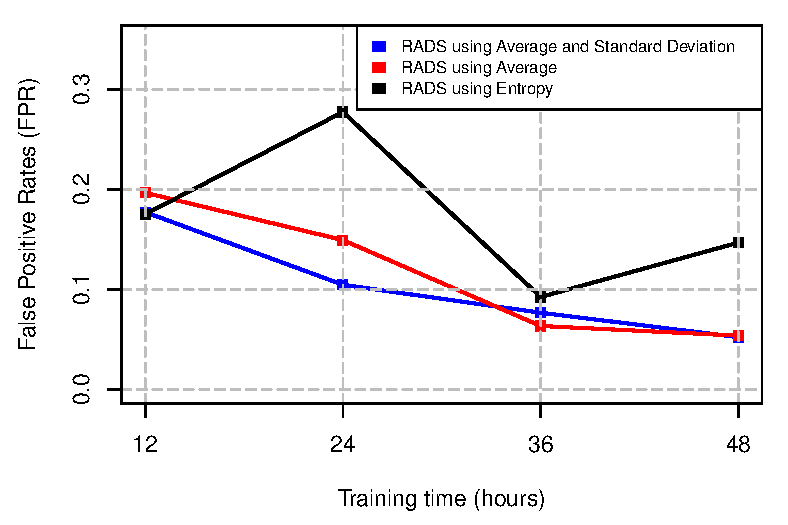
\epsfig{file = figures/offline_cpu_24, width = 0.7\columnwidth}}
      {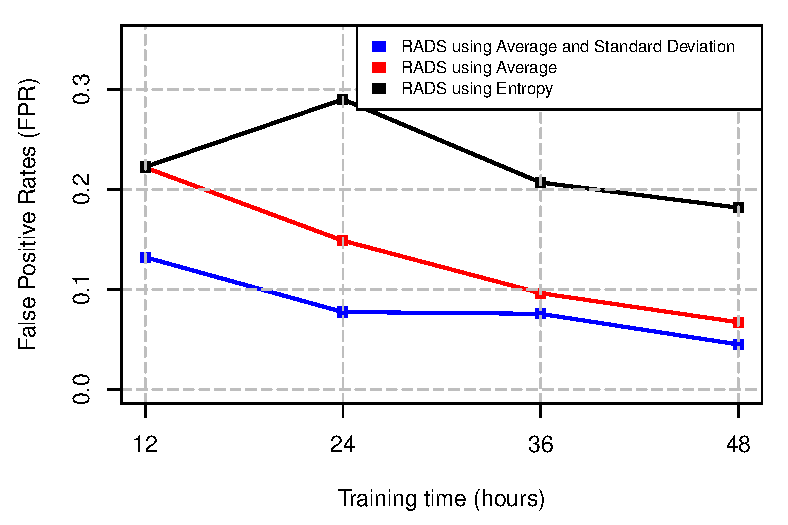
\epsfig{file = figures/offline_network_24, width = 0.7\columnwidth}}
     % {\epsfig{file = figures/offline_cpu_improvement, width = \columnwidth}}
   \caption{False Positive Rates (FPR) while running experiments on CPU utilisation (above) and network throughput (bottom)}
     % \caption{False positive rates of different versions of RAIDS while analysing CPU utilisation. (Below) Percentage of the performance improvement of RAIDS1/RAIDS2/RAIDS3 over average and entropy }
  \label{fig:offline_cpu_network}
 % \vspace{-0.1cm}
\end{figure}
%\vfill


%\subsubsection{Overall Performance of RADS}
\textbf{Overall Performance of RADS:}
%In the previous section we analysed the traces only from certain VMs in order to observe RAIDS responses towards varying Cloud workload behaviour. 
%We evaluate the overall performance of RAIDS in terms of dealing with the genuine workload spikes while analysing the traces chosen based on the selection process described in Section~\ref{sec:preparaiton_of_traces}. 
We evaluate the overall performance of RADS in terms of false positive rate. 
%by analysing the real-world Cloud workload traces. 
%chosen based on the selection process described in Section~\ref{sec:preparaiton_of_traces}. 
%This evaluation process considers different versions of RAIDS based on the number of artificial data points (required to deal with the genuine workload spikes as described in Section~\ref{sec:approach}) and the data pre-processing approach that it uses. The versions are defined in Table~\ref{tab:raids_versions}. Figure~\ref{fig:offline_cpu_network} presents the result of the False Positive Rates (FPR, calculated using the Equation~\ref{eq5}) of different versions of RAIDS while running tests on CPU utilisation trace of 82 VMs and network throughput trace of 212 VMs, which are collected from~\cite{workloadCCGRID:2015}. The tests are performed with 1 day (24 hours) of testing trace. Details of the training and the testing trace selection are presented in Section~\ref{sec:preparaiton_of_traces}.
%Specifically, in this evaluation process we performed different experiments for RADS based on the number of artificial data points and the data pre-processing approaches. The experiments are defined in Table~\ref{tab:raids_versions}. 
%As described in Section~\ref{sec:approach}, artificial data points are required to deal with the genuine workload spikes.  
%While describing the RADS framework in Section~\ref{sec:framework}, we consider the number of artificial data points to be equal to the total number of raw data points. To support this consideration, in this section we explore various numbers of artificial data points which are multiples of the total number of raw data points. 
% the optimal number of artificial data points for RAIDS. 
%The experiments with varying number of artificial data points are performed in order to decide the optimal number of artificial data points for RAIDS. 
Figure~\ref{fig:offline_cpu_network} presents the results of the False Positive Rates (FPR, calculated using Equation~\ref{eq5}) of RADS while running the experiments on a CPU utilisation trace of 82 VMs and a network throughput trace of 212 VMs.
%, 
%which are collected from~\cite{workloadCCGRID:2015}. 
%which were chosen based on the selection process described in Section~\ref{sec:preparaiton_of_traces}.
The experiments were performed with 24 hours of testing trace. 
%Details of the training and the testing trace selection process are presented in Section~\ref{sec:preparaiton_of_traces}.
%It is important to note that the traces from~\cite{workloadCCGRID:2015} does not include the information regarding the arrival processes, which can indicate the lifetime of user applications or VMs. Therefore, although the traces from~\cite{workloadCCGRID:2015} represent business critical workloads which generally use the same VM for a long period of time, we cannot verify whether the VMs under examination validate the assumption that we made in Section~\ref{sec:preparaiton_of_traces}: \textit{throughput the lifetime of the trace collection each monitored VM executed only a single application and that application continued to run in the same VM}. 
%Thus, the result that is presented in Figure~\ref{fig:offline_cpu_network} may not evaluate the performance of RAIDS correctly for the VMs which run variable or inconsistent user applications.
%we are not sure about which of the VMs under our examination run the same user application throughput the experimental period of 3 days. Thus, the result that is presented in Figure~\ref{fig:offline_cpu_network} may not evaluate the performance of RAIDS correctly for the VMs which run variable or inconsistent user applications. }
%the information regarding the Cloud applications running inside the selected VMs are not known and therefore its not 
% Similarly, Figure~\ref{fig:offline_network} presents the result of the FPR of different versions of RAIDS while analysing network throughput trace of 212 VMs collected from~\cite{workloadCCGRID:2015}. 
%The figures also present the percentage of the performance improvement (in terms of dealing with false positives) of RAIDS1/RAIDS2/RAIDS3 (we chose the best one amongst these in each occasion) over average and entropy.
We summarise the observations from the results as follows:
\begin{enumerate}[{(a)}]
%\item In case of both the experiments running on CPU utilisation and network throughput trace, all the versions of RAIDS achieve better performance (lower value of FPR means better performance) with the increase in the training time. This emphasises further the requirement of the proposed Training Optimiser Algorithm (Algorithm~\ref{raids_algorithm_training_optimiser}), which can decide the optimal training time.
%\item Results obtained from running experiments on both CPU utilisation and network throughput trace show that in most occasions RAIDS achieves better performance (lower value of FPR means better performance) with increase in training time and at one stage (training time - from $36$ to $48$ hours) the performance starts becoming stable. These results emphasise further the requirement of the proposed Training Optimiser Algorithm (Algorithm~\ref{raids_algorithm_training_optimiser}), which can decide the optimal training time.
\item On most occasions, when RADS uses its window-based time series analysis (combination of average and standard deviation), it achieves better performance (lower value of FPR means better performance) with increase in training time and at one stage (training time - from $36$ to $48$ hours) the performance starts becoming stable. These results emphasise further the requirement of the proposed training optimisation algorithm (Algorithm~\ref{raids_algorithm_training_optimiser}), which can decide the optimal training time.
\item The performance of RADS while using its window-based time series analysis is better than the performance of RADS while using average and entropy based analysis on most occasions.
% except for training time $36$ hours in case of CPU utilisation analysis where average based analysis performs slightly better than the window-based time series analysis of RADS. }
%\item The performance of RADS in case of RADS1, RADS2, and RADS3 (all using the proposed data pre-processing approach based on average and standard deviation) is better than the performance of RADS in case of AVG (using the average based data pre-processing approach) and ENT (using the entropy based data pre-processing approach) on most occasions (training time - $24, 36, 48$ hours). The performance of RADS is always better in case of RADS1 (using 1x of raw data points as artificial data points) in comparison to the performance of RADS in case of AVG and ENT except for one occasion (training time - 36 hours in case of CPU utilisation) when the performance slightly degrades. 
%This observation along with the fact that the more the artificial data points RADS uses the more computation resource and time it will require for the training supports the use of 1x of raw data points as artificial data points, 
%\item The performance of RADS in case of RADS1, RADS2, and RADS3 (all using the proposed data pre-processing approach based on average and standard deviation) is better than the performance of RADS in case of AVG (using the average based data pre-processing approach) and ENT (using the entropy based data pre-processing approach) on most occasions (training time - $24, 36, 48$ hours). The performance of RADS is always better in case of RADS1 (using 1x of raw data points as artificial data points) in comparison to the performance of RADS in case of AVG and ENT except for one occasion (training time - 36 hours in case of CPU utilisation) when the performance slightly degrades. This observation along with the fact that the more the artificial data points RADS uses the more computation resource and time it will require for the training supports the use of 1x of raw data points as artificial data points, 
%i.e. the number of artificial data points is equal to the total number of raw data points.
%i.e. there is no merit in using a number of artificial data points which is greater than the number of raw data points.
%Moreover, this investigation is important because using artificial data points which are manyfold of the total number of raw data points may improve the performance of RAIDS, but this may bring efficiency issues in terms of resource consumption and processing time. }
%However, none of the RAIDS version amongst RAIDS1, RAIDS2, and RAIDS3 is performing the best in all occasions and therefore, we had to choose the best amongst these in each occasion while comparing against AVG and ENT in the bar plots depicting the percentage of performance improvement. Due to the same reason we do not conclude which RAIDS version amongst RAIDS1, RAIDS2, and RAIDS3 is the best, instead we use RAIDS1 and allow the proposed Training Optimiser Algorithm (Algorithm~\ref{raids_algorithm_training_optimiser}) to decide the training data points with which it can be trained to perform successfully. Selecting only RAIDS1 
%\item In case of CPU utilisation analysis, RAIDS2 and RAIDS3 achieves better than AVG and ENT when the training time is between 24-48 hours, whereas RAIDS1 achieves  better than AVG and ENT in all occasions except for training time 36 hours. In case of network throughput analysis, RAIDS1 
%\item The performance improvement of RAIDS (RAIDS1/RAIDS2/RAIDS3) is much higher in case of network throughput analysis (31-49\% over average and 40-75\% over entropy) in comparison to the performance improvement of RAIDS in case of CPU utilisation analysis. 
\end {enumerate}

%As mentioned earlier, due to the limited knowledge of the traces, we could not choose the VMs which run the same application consistently throughout the data collection period. As a result, the traces analysed above may include VMs which run inconsistent Cloud applications.
%and may result in poor performance for RAIDS. 
%If RADS is applied only to VMs which run the same Cloud application consistently, RADS may achieve better performance than what is observed above. 

%% OFFLINE NEWORK ANALYSIS
%%\vfill
%\begin{figure}[!h]
%  %\vspace{-0.2cm}
%  \centering
%   {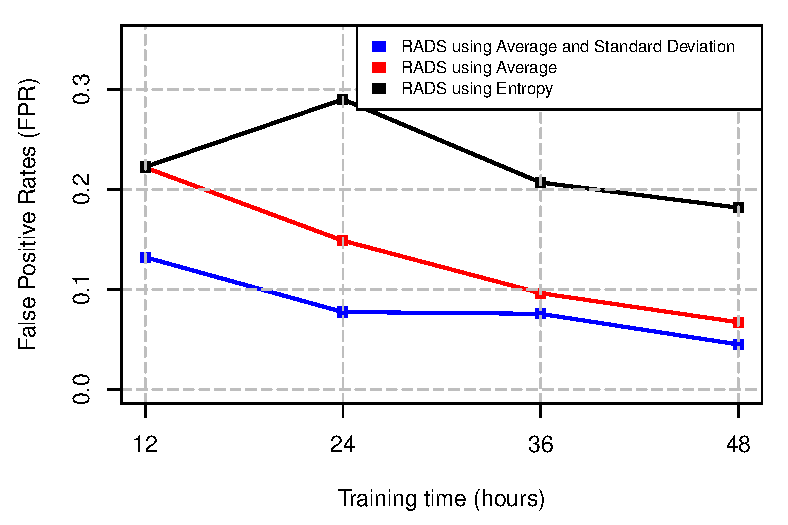
\epsfig{file = figures/offline_network_24, width = \columnwidth}}
%     % {\epsfig{file = figures/offline_network_improvement, width = \columnwidth}}
% %  \caption{(Above) False positive rates of different versions of RAIDS while analysing network throughput. (Below) Percentage of the performance improvement of RAIDS1/RAIDS2/RAIDS3 over average and entropy }
%    \caption{False positive rates of different versions of RAIDS while analysing network throughput}
%
%  \label{fig:offline_network}
% % \vspace{-0.1cm}
%\end{figure}
%%\vfill



